%Copyright 2011 Anthony Youd/Newcastle University
%
%   Licensed under the Apache License, Version 2.0 (the "License");
%   you may not use this file except in compliance with the License.
%   You may obtain a copy of the License at
%
%       http://www.apache.org/licenses/LICENSE-2.0
%
%   Unless required by applicable law or agreed to in writing, software
%   distributed under the License is distributed on an "AS IS" BASIS,
%   WITHOUT WARRANTIES OR CONDITIONS OF ANY KIND, either express or implied.
%   See the License for the specific language governing permissions and
%   limitations under the License.

\documentclass[12pt]{report}
\usepackage[a4paper,left=30mm,right=30mm,top=40mm,bottom=35mm]{geometry}
\setlength{\headheight}{15pt}
\usepackage{manual}

\begin{document}

  \manualtitle{The GPE Code}
              {Anthony~J.~Youd}
              {fig/trapvortex}
              {\small{Sat 09 Jul 16:32:45 2011}\\
               \tiny{\copyright Anthony J. Youd/Newcastle University 2011}}

%%%%%%%%%%%% START OF DOCUMENT CONTENT %%%%%%%%%%%%%%%%

  \input{licence}

  \pagenumbering{roman}

  \tableofcontents

  \clearpage

  \pagenumbering{arabic}

  % $Id$
%------------------------------------------------------------------------------

\begin{chapter}{\label{cha:introduction}Introduction}
\end{chapter}

  % $Id$
%------------------------------------------------------------------------------

\begin{chapter}{\label{cha:quickstart}Quick start guide}
  This chapter is intended as a quick start guide to help you compile, run and
  view the results of the GPE code.  More detailed information about various
  technical aspects of the code can be found in chapter SOMETHING OR OTHER;
  here we will outline the basics of going through a run cycle, by using the
  provided \gpeexample{ring} example.

  This example propagates a vortex ring in a homogeneous condensate for a short
  time.

  \section{Setting the run parameters and initial condition}
  Change to the \gpefile{examples/ring} directory.  In here, you
  will find symbolic links to the source files, and in addition, three
  \gpefile{.in} files.  In general, it is these files ---
  \gpefile{parameters.in}, \gpefile{ic.in}, and \gpefile{run.in} --- which you
  will need to edit in order to set up a run.

  \subsection{parameters.in}
  For this example, simply change \gpevar{nyprocs} and \gpevar{nzprocs}, so
  that \gpevar{nyprocs*nzprocs} is equal to (or less than) the number of
  processors on your machine.  If memory is an issue, then you may want to
  reduce any or all of \gpevar{nx}, \gpevar{ny}, or \gpevar{nz} (and possibly
  \gpevar{xr}, \gpevar{yr}, and \gpevar{zr} below).  See
  section~\ref{subsec:parameters.in} for a full description of this file.  

  \subsection{ic.in}
  This file defines the initial condition.  For this example, no changes are
  necessary.  See section~\ref{subsec:ic.in} for a full description of this
  file.

  \subsection{\label{subsec:runin}run.in}
  This file defines the main parameters for the run, as a set of Fortran
  \verb"namelist"s.
  
  For the \gpeexample{ring} example, the parameters are correctly set.  You
  might want to alter \gpevar{end\_time} if the run takes too long.  If you
  altered any of \gpevar{nx}, \gpevar{ny}, or \gpevar{nz} in
  \gpefile{parameters.in}, then you might also want to alter \gpevar{xr},
  \gpevar{yr}, or \gpevar{zr} as appropriate.  These parameters set the
  right-hand end of the physical extent of the computational box (the left-hand
  end is set to the same value with opposite sign).  See
  section~\ref{subsec:run.in} for a full description of this file.

  \section{Compiling the code}
  Choose a directory where your run will take place (we shall assume the
  directory \verb"run_dir" in what follows).  This directory should not be on a
  network file system (NFS), which will likely be too slow (and under quota
  restrictions).  The \gpeexample{ring} example will require approximately 3GB
  of disk space with the default parameters.

  Now compile the code with
  %
  \begin{Verbatim}
    ./setup run_dir
  \end{Verbatim}
  %
  This will compile the code\footnote{The default Makefile assumes the sunf95
  compiler is available and in the path, and that 64-bit code should be
  generated.  If this is not what you want, then you will need to edit the
  Makefile.  See section~\ref{sec:makefile} for more information.}, create the
  directory \verb"run_dir", and copy \gpefile{parameters.in}, \gpefile{ic.in},
  \gpefile{run.in}, and \gpefile{run.sh} to the run directory.  In addition,
  the executable \gpefile{gpe} is moved to the run directory.

  This run uses double-precision floating-point arithmetic.  For other runs, if
  you require only single precision, then remember to set \gpevar{pr}
  appropriately in \gpefile{parameters.in}, and compile with
  %
  \begin{Verbatim}
    ./setup run_dir single
  \end{Verbatim}
  %
  Now change to the run directory ready to run the code.

  \section{Running the code}
  To run the code simply type
  %
  \begin{Verbatim}
    ./run.sh <nprocs>
  \end{Verbatim}
  %
  where \verb"<nprocs>" specifies on how many processes the code should run.
  Ideally, this should be less than or equal to the number of physical
  processors in your system.  It should match \gpevar{nyprocs*nzprocs} in
  \gpefile{parameters.in}, otherwise an error will result.  The job is run in
  the background using \verb"nohup", so control immediately returns to the
  terminal, and logging out of the machine on which the job is running will not
  terminate the job.

  The \gpefile{run.sh} script has several options for controlling how the run
  should be started.  Run it with no arguments to see usage instructions.

  \section{During the run}
  As a first sanity check that the job is running, look for a file called
  \gpefile{ERROR} in the run directory.  If this does not exist, then that is a
  good sign.  Also have a look at the file \gpefile{log.txt}; this should say
  something like
  %
  \begin{Verbatim}
  Explicit fifth order Runge-Kutta-Fehlberg adaptive time stepping
  Homogeneous condensate, natural units non-dim.
  -2i*dpsi/dt + 2iU*dpsi/dx = del^2(psi) + (1-|psi|^2)psi
  \end{Verbatim}
  %
  and is something to check to make sure the correct time stepping scheme is
  being used, and that the correct form of the GPE is being solved.

  The command \verb"top" should show the \gpefile{gpe} executable listed the
  same number of times as the number of processes on which you chose to run the
  job.

  Finally, if numbers are appearing in the \gpefile{*.dat} files, then you can
  at least be sure that the job is running.

  \section{Important run-time files}
  \subsection{The RUNNING file}
  When the job is running there is an empty file called \gpefile{RUNNING} in
  the run directory; when the job is finished this file is deleted.  You can
  also delete this file at any time to immediately stop the run cleanly.  The
  job should never be ended by using \verb"kill" or \verb"killall", unless an
  unrecoverable error occurs.

  \subsection{The ERROR file}
  If a serious error occurs which the code can anticipate, then the
  \gpefile{ERROR} file is created in the run directory.  Its contents will
  provide details of the error.  The job will be terminated cleanly in this
  case, and the \gpefile{RUNNING} file will be removed.

  \subsection{The log.txt file}
  Any output that the job would normally print to the screen is instead
  redirected to the file \gpefile{log.txt}.  It is a good idea to periodically
  check this file to make sure that no unexpected run-time errors have
  occurred.  Any errors which are written to \gpefile{ERROR} are also written
  to this file.  Any errors which the code could not anticipate, such as MPI
  communication errors, will appear here.  In this case the job will most
  likely not terminate cleanly, and the \gpefile{RUNNING} file might not be
  removed.

  \subsection{The SAVE file}
  As the job is running, data are periodically saved, according to the
  \gpevar{save\_rate} parameters in \gpefile{run.in}.  Every time step, the
  code checks for the existence of a file called \gpefile{SAVE} in the run
  directory.  If this file exists, then 3D data (from which isosurfaces and
  contour plots can be produced) is immediately written to disk.  The
  \gpefile{SAVE} file is then automatically removed.  This file can be created,
  for example, by using the \verb"touch" command, \ie \verb"touch SAVE".

  \section{Program output}
  Once a job has started, the code produces various output files containing
  various data.  Exactly which files appear depends on which parameters have
  been set in the \gpevar{io\_params} namelist in \gpefile{run.in}.

  The numbered \gpefile{proc} directories contain data local to each process on
  which the job is running.  This is where 3D isosurface data are stored.

  A full description of the output files is given in chapter SOMETHING OR
  OTHER.

  \section{\label{sec:viewing_results}Viewing results}
  During and after a run it is possible to plot various 1D graphs, 2D contour
  plots and 3D isosurfaces.  For the 1D time-series graphs, gnuplot is a good
  program to use (although nearly any plotting program capable of understanding
  simple columnar text files will be sufficient).  This section will describe
  how to produce some plots.
  
  \subsection{1D time-series plots}
  1D time-series data is produced in the \gpefile{*.dat} files at the top-level
  of the run directory, much of which is self-explanatory, given the names of
  the files, \eg \gpefile{energy.dat}, \gpefile{mass.dat}.  A full description
  of what can be found in these data files is given in chapter SOMETHING OR
  OTHER, but note that the exact contents of files can be subject to change.
  
  So, for the \gpeexample{ring} example, using gnuplot to plot the total energy
  in the system, you could do
  %
  \begin{Verbatim}
    p "energy.dat" u 1:3 w lp
  \end{Verbatim}
  %
  which will plot column three (line length) versus column one (real time) in
  the file, and where the \verb"plot", \verb"using", \verb"with", and
  \verb"linespoints" keywords have been abbreviated to the shortest
  non-ambiguous form, which is possible with any gnuplot command.

  As it turns out, there are not many interesting 1D graphs for the
  \gpeexample{ring} example!

  \subsection{\label{subsec:contour_plots}Contour plots}
  Contour and isosurface data are stored in binary form within the
  \gpefile{proc} directories; the layout of the binary files is explained in
  chapter SOMETHING OR OTHER.

  If you have access to the Interactive Data Language (IDL) graphics program,
  then IDL routines are provided with the code to directly plot the data.
  These are located in the \gpefile{idl} subdirectory of the main code
  directory.

  From the run directory start IDL with the command \verb"idl".  Providing the
  IDL environment is set up correctly (see section~\ref{subsec:idl_setup}) you
  should be able to type
  %
  \begin{Verbatim}
    gpe, 0, 0, /dbl, /cntr
  \end{Verbatim}
  %
  which will show a contour plot of the density of the initial condition as a
  slice through the $(x,y)$-plane at $z=0$.  You should get something which
  looks like figure~\ref{fig:ring_ic_con}.
  %
  \begin{figure}
    \centering
    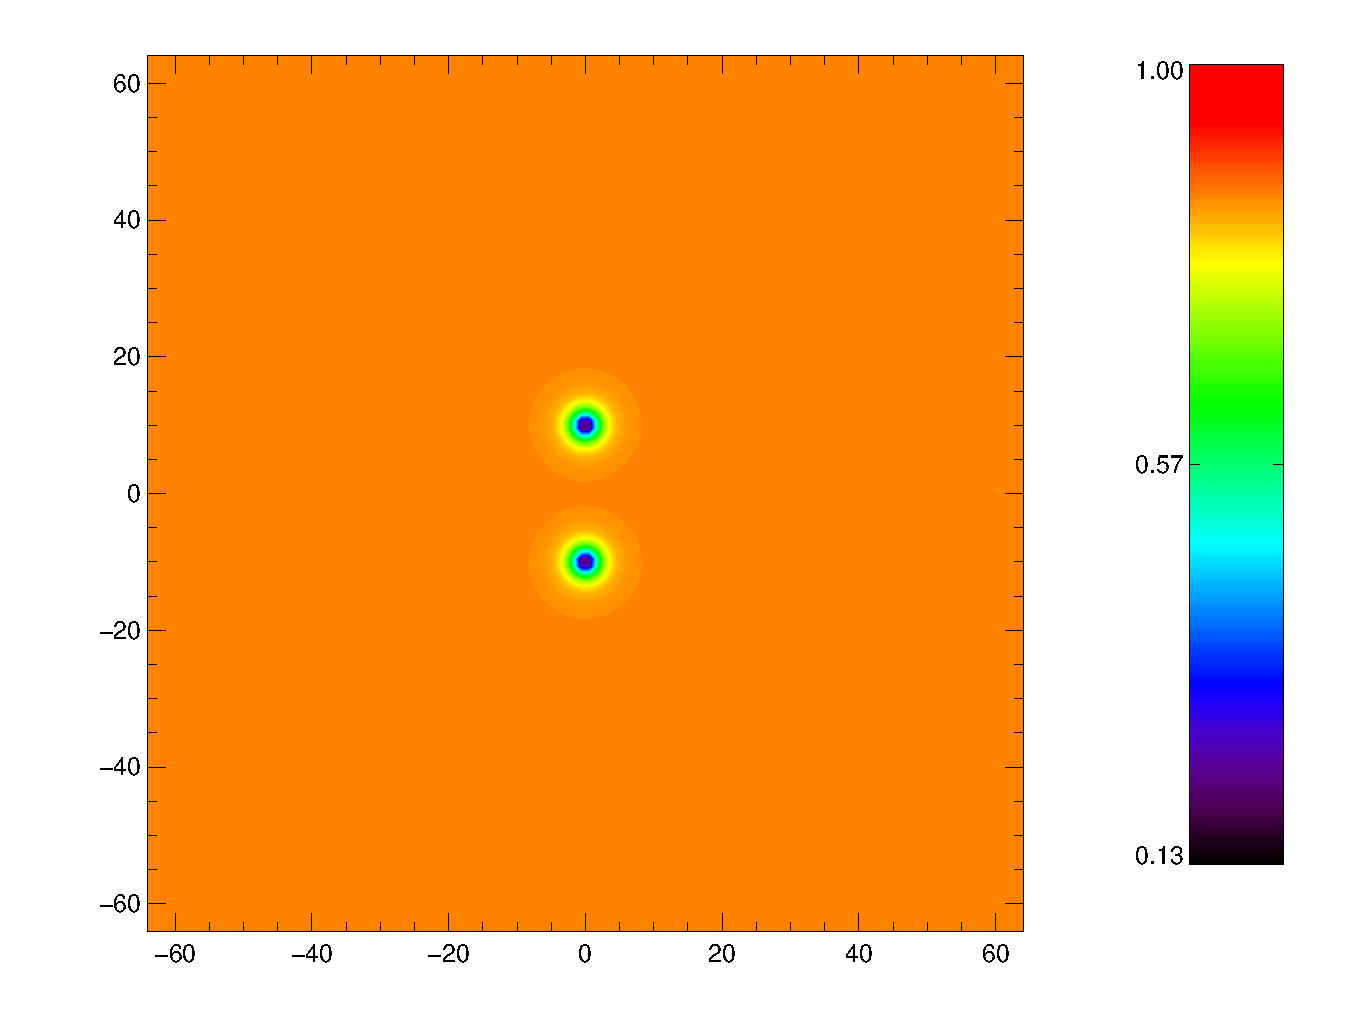
\includegraphics[scale=0.5]{fig/ring_ic_con}
    \caption{\label{fig:ring_ic_con}Contour plot of the density of a vortex
      ring of radius $R_{0}=10$ in the $(x,y)$-plane at $z=0$.}
  \end{figure}
  %
  The word \gpevar{gpe} represents an IDL program, which takes two non-optional
  arguments.  The first is the index corresponding to the first file you want
  to plot, and the second is the index corresponding to the last file you want
  to plot.  \emph{Important: For output to the screen these numbers should
  always be the same.}

  The numbers refer to the files within the \gpefile{proc} directories.  If you
  look in \gpefile{proc00}, for example, you will see a number of files named
  \gpefile{dens*******.dat}.  The arguments to \gpevar{gpe} are the numbers
  within the filenames, excluding the leading zeroes.

  So, \gpevar{gpe, 0, 0} plots \gpefile{dens0000000.dat}; \gpevar{gpe, 334,
  334} plots \gpefile{dens0000331.dat}, etc.

  The remaining arguments are optional.  The first, \gpevar{/dbl}, denotes that
  the binary data are double-precision.  You must always provide this switch
  when you have performed a double-precision run.  In a single-precision run,
  this switch is not necessary.

  The second, \gpevar{/cntr}, is a switch which turns on contour output, rather
  than the default, which is an isosurface (see
  section~\ref{subsec:isosurface_plots}).

  To quit IDL at any time type \verb"exit".

  \subsection{\label{subsec:isosurface_plots}Isosurface plots}
  Start IDL again, and do exactly as in section~\ref{subsec:contour_plots}, but
  this time leave off the \gpevar"/cntr" switch.
  
  You should see an isosurface plot in a window similar to that in
  figure~\ref{fig:ring_ic_iso}, and a control panel with various buttons on it.
  Most of the control panel buttons can be ignored.  The \verb"bbox",
  \verb"content", and \verb"axis" buttons turn on or off the bounding box, the
  content, and the axes labels respectively.  You will need to click the
  \verb"Redraw" button if you make any changes.
  %
  \begin{figure}
    \centering
    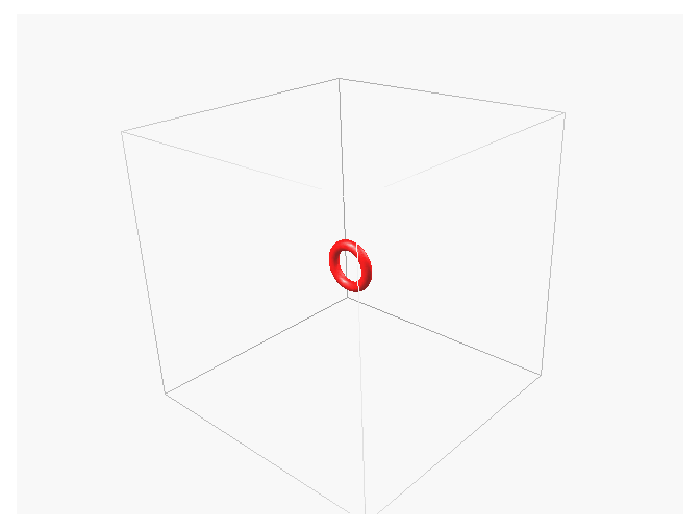
\includegraphics[scale=1]{fig/ring_ic_iso}
    \caption{\label{fig:ring_ic_iso}Isosurface plot of the density of a vortex
      ring of radius $R_{0}=10$ at the level $\abs{\psi}^{2} = 0.75$.}
  \end{figure}
  %
  Left-click and hold in the white window and you can move the view around;
  right-clicking zooms in and out, and middle-clicking moves the centre
  viewpoint.  Depending on the speed of your machine, and the complexity of the
  displayed image, zooming and moving the view might be a little slow, so move
  the mouse slowly, and avoid large jerky movements.

  The coloured bar in the control panel is a histogram of the density, and
  clicking in here will redraw the isosurface at the new density level, which
  is shown toward the right-hand side of the control panel.

  Pressing \verb"auto" will automatically redraw the isosurface when other
  boxes are checked, for example, the axes, or whether the surface is solid,
  wireframe, or a series of points.  If the display is too slow, selecting
  \verb"points" or \verb"wireframe" instead of \verb"solid" will speed it up.

  \subsection{Animations}
  By saving a series of snapshots of 2D or 3D data it is possible to then
  combine them into an animation.

  From the run directory run the script \gpefile{create-links}.  This will
  create a directory \gpefile{links}, which contains renamed symbolic links
  (shortcuts) pointing to the isosurface files within each process directory.
  This is to make sure that the files are numbered sequentially in steps of
  one.  The \gpefile{create-links} script is located in the \gpefile{scripts}
  subdirectory of the main code directory.  Giving it the argument
  \gpefile{--help} will provide usage instructions.

  \subsubsection{Contour animations}
  Change to the links directory and create another directory called
  \gpefile{images}, then start IDL again.

  Now type
  %
  \begin{Verbatim}
    gpe, 0, 9, /dbl, /cntr, /c_anim
  \end{Verbatim}
  %
  This will loop over all data files numbered 0 to 9 and save
  \verb"con_dens*******.png" files in the \gpefile{images} directory.  (If you
  left the \gpeexample{ring} example parameters at their defaults, then you
  should actually find 100 data files in each \gpefile{proc} directory, so you
  could do plots from 0 to 99 if you wish.)

  \emph{If you miss off the /c\_anim switch here, you will get all the
  plots shown to the screen.  When you are plotting 100 or more files, this
  can be very bad and in some cases might run your machine out of memory.}

  Now change to the \verb"images" directory and run the \gpefile{makemovie}
  script, which is located in the \gpefile{scripts} subdirectory of the main
  code directory:
  %
  \begin{Verbatim}
    makemovie -i png -p con_dens
  \end{Verbatim}
  %
  which will create an AVI animation out of the PNG files, with 10 frames,
  saving the output as \gpefile{output.avi}.

  You can then play the animation with any media player, for example,
  %
  \begin{Verbatim}
    mplayer output.avi
  \end{Verbatim}
  %
  The animation is very short; if it works you can try a longer animation by
  repeating the \gpevar{gpe} IDL command with arguments 0 and 99.

  \subsubsection{Isosurface animations}
  Rename the \gpefile{images} directory to something else, and recreate an
  empty \gpefile{images} directory.  Start IDL and this time type
  %
  \begin{Verbatim}
    gpe, 0, 9, /png
  \end{Verbatim}
  %
  As for the contour plots before, this will save PNG files in the
  \gpefile{images} directory, which you can then convert into an animation
  using \gpefile{makemovie}.

  \emph{If you miss off the /png switch, all the output will again go to the
  screen.  This should be avoided if possible.}

  \section{\label{sec:restart}Restarting the code}
  After a run, you might decide that you would like to restart the code from
  where you left off, for example, maybe you started your run in imaginary
  time, and now want to switch to real time, or maybe you did not run for quite
  long enough.

  If this is the case, create a new directory where the restarted run will take
  place, and copy \gpefile{parameters.in}, \gpefile{ic.in}, \gpefile{run.in},
  \gpefile{run.sh}, and the executable \gpefile{gpe} from the initial run
  directory to the restart directory.

  Now edit \gpefile{run.in}, change \gpevar{restart} to \gpevar{.true.}, and
  make any other changes necessary.  Recompilation is not needed when making
  changes only to \gpefile{run.in}.

  Now type
  %
  \begin{Verbatim}
    ./run.sh -r <initial run directory> <nprocs>
  \end{Verbatim}
  %
  where \verb"<initial run directory>" is the directory of the run which you
  want to continue.  This will copy the \gpefile{end\_state.dat} files from the
  \gpefile{proc} directories to the restart directory (suitably renamed).  The
  \gpefile{log.txt} file should then report that the code is
  %
  \begin{Verbatim}
    Getting restart conditions
  \end{Verbatim}
  %
  and will restart from where it left off.
\end{chapter}

  % $Id: equations.tex 604 2010-06-09 11:24:10Z najy2 $
%------------------------------------------------------------------------------

\begin{chapter}{\label{cha:equations}Governing equations, boundary conditions
  and non-dimensionalisation}

  The single-particle complex wavefunction $\psi(\vec{r}, t)$ for $N$ bosons of
  mass $m$ obeys the 3 dimensional, time dependent Gross--Pitaevskii (GP)
  equation \citep{Gross61,Pitaevskii61}
  %
  \begin{equation}
    \eye \hbar \frac{\pa \psi}{\pa t} = -\frac{\hbar^{2}}{2m} \nabla^{2} \psi +
    \Vtrap \psi + g \left|\psi\right|^{2} \psi - \mu \psi,
  \end{equation}
  %
  where $\hbar$ is Planck's constant, $\Vtrap$ is an external potential, $g$ is
  the strength of the interactions between the bosons, and $\mu$ is the
  chemical potential.

  It describes the evolution of the ground state of a quantum system of weakly
  interacting bosons, in the limit of zero temperature, and when the number of
  bosons $N$ is large.

  \begin{equation}
    \kappa = \frac{h}{m} = \frac{2\pi\hbar}{m}
    \label{eqn:one}
  \end{equation}

  \noindent Then
  %
  \begin{equation}
    \kappa^{*} = \frac{\hbar/(2\mu)}{a^{2}}\kappa = \frac{\hbar}{2\mu
      a^{2}}\kappa
    \label{eqn:two}
  \end{equation}
  %
  Then substituting \eqref{eqn:two} into \eqref{eqn:one} gives
  %
  \begin{equation*}
    \begin{aligned}
      \frac{2\mu a^{2}}{\hbar}\kappa^{*} &= \frac{2\pi\hbar}{m} \\
      \implies \kappa^{*} &= \frac{2\pi\hbar}{m} \frac{\hbar}{2\mu a^{2}} \\
      &= \frac{2\pi\hbar^{2}}{2m\mu a^{2}}
    \end{aligned}
  \end{equation*}
  %
  Then using $a^{2} = \hbar^{2}/(2m\mu)$ gives $\kappa^{*} = 2\pi$.
\end{chapter}

  %Copyright 2011 Anthony Youd/Newcastle University
%
%   Licensed under the Apache License, Version 2.0 (the "License");
%   you may not use this file except in compliance with the License.
%   You may obtain a copy of the License at
%
%       http://www.apache.org/licenses/LICENSE-2.0
%
%   Unless required by applicable law or agreed to in writing, software
%   distributed under the License is distributed on an "AS IS" BASIS,
%   WITHOUT WARRANTIES OR CONDITIONS OF ANY KIND, either express or implied.
%   See the License for the specific language governing permissions and
%   limitations under the License.

\begin{chapter}{\label{cha:numerics}Numerical formulation}

  This chapter outlines the numerical formulation which is used to solve the
  GPE.  Time stepping is performed explicitly using a choice of schemes, and
  spatial discretisation is performed with either second- or fourth-order
  centred finite differences.

  \section{Time stepping}
  As briefly mentioned in the introduction, a choice of time stepping schemes
  is possible.  Each of these is explained in this section.

  \subsection{Euler's method}
  For a general partial differential equation of the form
  %
  \begin{equation*}
    \frac{\pa \psi}{\pa t} = f(\psi, \vec{r}, t),
  \end{equation*}
  %
  where $f$ is some function representing the right hand side of the equation,
  Euler's method is
  %
  \begin{equation*}
    \psi^{p+1} = \psi^{p} + \dt f^{p} + \mathcal{O}(\dt^{2}),
  \end{equation*}
  %
  where $\dt$ is the time step, $\psi^{p} = \psi\left( x, y, z, t^{p}\right)$,
  $t^{p} = p\dt$, and $f^{p} = f\left( \psi^{p} \right)$.

  This scheme is only first order accurate in $\dt$, and is not recommended for
  use, other than for very rough testing.  It can be selected in the code by
  setting the parameter \gpevar{scheme} equal to \verb"euler" in
  \gpefile{run.in}.

  \subsection{Second-order Runge--Kutta method}
  The second-order Runge--Kutta method (also known as the midpoint method) is
  second order accurate in time, and takes the form
  %
  \begin{equation*}
    \psi^{p+1} = \psi^{p} + \dt k_{2} + \mathcal{O}(\dt^{3}),
  \end{equation*}
  %
  where
  \begin{equation*}
    \begin{aligned}
      k_{1} &= f\left( t^{p}, \psi^{p} \right), \\
      k_{2} &= f\left( t^{p+\frac{1}{2}}, \psi^{p} + \frac{1}{2}\dt k_{1}
      \right).
    \end{aligned}
  \end{equation*}
  %
  This scheme can be selected by setting \gpevar{scheme} equal to \verb"rk2".

  \subsection{Fourth-order Runge--Kutta method}
  The fourth-order Runge--Kutta method is fourth order accurate in time and
  takes the form
  %
  \begin{equation*}
    \psi^{p+1} = \psi^{p} + \dt \left( \frac{k_{1}}{6} + \frac{k_{2}}{3} +
    \frac{k_{3}}{3} + \frac{k_{4}}{6} \right) + \mathcal{O}(\dt^{5}),
  \end{equation*}
  %
  where
  \begin{equation*}
    \begin{aligned}
      k_{1} &= f\left( t^{p}, \psi^{p} \right), \\
      k_{2} &= f\left( t^{p+\frac{1}{2}}, \psi^{p} + \frac{1}{2}\dt k_{1}
      \right), \\
      k_{3} &= f\left( t^{p+\frac{1}{2}}, \psi^{p} + \frac{1}{2}\dt k_{2}
      \right), \\
      k_{4} &= f\left( t^{p+1}, \psi^{p} + \dt k_{3} \right).
    \end{aligned}
  \end{equation*}
  %
  This scheme can be selected by setting \gpevar{scheme} equal to \verb"rk4".

  \subsection{Runge--Kutta--Fehlberg method}
  The Runge--Kutta--Fehlberg method is a hybrid fourth/fifth order adaptive
  time stepping scheme.  In the code, the fifth-order formula is
  %
  \begin{equation*}
    \begin{aligned}
      k_{1} &= \dt f\left( t^{p}, \psi^{p} \right), \\
      k_{2} &= \dt f\left( t^{p} + a_{2}\dt, \psi^{p} + b_{21} k_{1}
        \right), \\
      k_{3} &= \dt f\left( t^{p} + a_{3}\dt, \psi^{p} + b_{31} k_{1} + b_{32}
        k_{2} \right), \\
      k_{4} &= \dt f\left( t^{p} + a_{4}\dt, \psi^{p} + b_{41} k_{1} + b_{42}
        k_{2} + b_{43} k_{3} \right), \\
      k_{5} &= \dt f\left( t^{p} + a_{5}\dt, \psi^{p} + b_{51} k_{1} + b_{52}
        k_{2} + b_{53} k_{3} + b_{54} k_{4} \right), \\
      k_{6} &= \dt f\left( t^{p} + a_{6}\dt, \psi^{p} + b_{61} k_{1} + b_{62}
        k_{2} + b_{63} k_{3} + b_{64} k_{4} + b_{65} k_{5} \right), \\
      \psi^{p+1} &= \psi^{p} + c_{1} k_{1} + c_{2} k_{2} + c_{3} k_{3} + c_{4}
        k_{4} + c_{5} k_{5} + c_{6} k_{6} + \mathcal{O}(\dt^{6}).
    \end{aligned}
  \end{equation*}
  %
  The embedded fourth-order formula is given by
  %
  \begin{equation*}
    \psi_{*}^{p+1} = \psi^{p} + c_{1}^{*} k_{1} + c_{2}^{*} k_{2} + c_{3}^{*}
    k_{3} + c_{4}^{*} k_{4} + c_{5}^{*} k_{5} + c_{6}^{*} k_{6} +
    \mathcal{O}(\dt^{5}),
  \end{equation*}
  %
  so that an error estimate can be obtained with
  %
  \begin{equation*}
    \Delta \equiv \psi^{p+1} - \psi_{*}^{p+1} = \sum_{i=1}^{6}{\left( c_{i} -
    c_{i}^{*} \right) k_{i}}.
  \end{equation*}
  %
  The values of the constants are those given by \citet{CK90}, and are
  reproduced here in table~\ref{tab:cash_karp}.
  %
  \begin{table}
    \renewcommand{\arraystretch}{1.5}
    \centering
    \begin{tabular}{|c|c|ccccc|c|c|}
      \hline
      $i$ & $a_{i}$ & \multicolumn{5}{c|}{$b_{ij}$} & $c_{i}$ & $c_{i}^{*}$ \\
      \hline
      $1$ & & & & & & & $\frac{37}{378}$ & $\frac{2825}{27648}$ \\
      $2$ & $\frac{1}{5}$ & $\frac{1}{5}$ & & & & & $0$ & $0$ \\
      $3$ & $\frac{3}{10}$ & $\frac{3}{40}$ & $\frac{9}{40}$ & & & & $\frac{250}{621}$ & $\frac{18575}{48384}$ \\
      $4$ & $\frac{3}{5}$ & $\frac{3}{10}$ & $-\frac{9}{10}$ & $\frac{6}{5}$ & & & $\frac{125}{594}$ & $\frac{13525}{55296}$ \\
      $5$ & $1$ & $-\frac{11}{54}$ & $\frac{5}{2}$ & $-\frac{70}{27}$ & $\frac{35}{27}$ & & $0$ & $\frac{277}{14336}$ \\
      $6$ & $\frac{7}{8}$ & $\frac{1631}{55296}$ & $\frac{175}{512}$ & $\frac{575}{13824}$ & $\frac{44275}{110592}$ & $\frac{253}{4096}$ & $\frac{512}{1771}$ & $\frac{1}{4}$ \\
      \hline
      \multicolumn{2}{|c}{$j=$} & $1$ & $2$ & $3$ & $4$ & \multicolumn{1}{c}{5} & \multicolumn{2}{c|}{} \\
      \hline
    \end{tabular}
    \caption{\label{tab:cash_karp}The Cash--Karp constants for the
      Runge--Kutta--Fehlberg scheme.}
  \end{table}
  %
  Full details of the algorithm can be found in Numerical Recipes \citep[\S
  16.2, p.708,][]{NR92}.

  This scheme can be selected by setting \gpevar{scheme} equal to \verb"rk45".

  \section{Spatial discretisation}
  Centred finite differences are used to spatially discretise the GPE; these
  can be either second or fourth order.

  For a general partial differential equation of the form
  %
  \begin{equation*}
    \frac{\pa \psi}{\pa t} = f(\psi, \vec{r}, t),
  \end{equation*}
  %
  where $f$ is some function representing the right hand side of the equation,
  the spatial discretisation takes the form
  %
  \begin{equation*}
    \frac{\pa \psi_{ijk}}{\pa t} = f_{ijk},
  \end{equation*}
  %
  where $\psi_{ijk} = \psi\left( x_{i}, y_{j}, z_{k}, t \right)$, $x_{i} =
  i\dx$, $y_{j} = j\dy$, $z_{k} = k\dz$, and $f_{ijk} = f\left( \psi_{ijk}
  \right)$.

  \subsection{Second-order finite differences}
  The second-order finite-difference approximation to the first derivative,
  with respect to $x$, is given by
  %
  \begin{equation*}
    \frac{\pa \psi}{\pa x} \approx \frac{\psi_{i+1} - \psi_{i-1}}{2\dx},
  \end{equation*}
  %
  where we have dropped the $j$ and $k$ indices for clarity.

  Similarly, the second-order approximation to the second derivative is
  %
  \begin{equation*}
    \frac{\pa^{2} \psi}{\pa x^{2}} \approx \frac{\psi_{i+1} - 2\psi_{i} +
    \psi_{i-1}}{\dx^{2}}.
  \end{equation*}
  %
  Second-order finite differences can be chosen by setting \gpevar{order} equal
  to \verb"2" in \gpefile{run.in}.

  \subsection{Fourth-order finite differences}
  The fourth-order finite-difference approximation to the first derivative,
  with respect to $x$, is given by
  %
  \begin{equation*}
    \frac{\pa \psi}{\pa x} \approx \frac{-\psi_{i+2} +8\psi_{i+1} - 8\psi_{i-1}
    + \psi_{i-2}}{12\dx}.
  \end{equation*}
  %
  Similarly, the fourth-order approximation to the second derivative is
  %
  \begin{equation*}
    \frac{\pa^{2} \psi}{\pa x^{2}} \approx \frac{-\psi_{i+2} + 16\psi_{i+1} -
    30\psi_{i} + 16\psi_{i-1} - \psi_{i-2}}{12\dx^{2}}.
  \end{equation*}
  %
  Fourth-order finite differences can be chosen by setting \gpevar{order} equal
  to \verb"4".

  \section{Boundary conditions}
  The code implements both periodic and reflective boundary conditions.  Since
  both of these conditions are behavioural, rather than numerical, no boundary
  conditions are explicitly set on $\psi$ itself.  Note that it is not possible
  to mix boundary conditions yet.

  \subsection{Periodic boundary conditions}
  Suppose the $x$-coordinate runs from $x_{0}$ to $x_{n}$.  Then clearly the
  values of $\psi$ at $x_{-1}$ and $x_{n+1}$ are needed to compute a first
  derivative, for example.

  Periodic boundary conditions are implemented such that
  %
  \begin{equation*}
    \begin{aligned}
      x_{-1}  &= x_{n}, \\
      x_{n+1} &= x_{0}.
    \end{aligned}
  \end{equation*}
  %
  These conditions are also applied in the $y$- and $z$-directions, and can be
  naturally extended for higher order approximations.

  To use periodic boundary conditions set \gpevar{bcs} equal to \verb"1" in
  \gpefile{run.in}.

  \subsection{Reflective boundary conditions}
  The physical meaning of reflective boundary conditions is that structures
  within the computational box see images of themselves across the box
  boundaries.  This would cause a vortex ring to annihilate on approaching a
  boundary, for example, as it sees an image of itself approaching the boundary
  from the opposite direction (outside the computational box).

  These boundary conditions are implemented such that
  %
  \begin{equation*}
    \begin{aligned}
      x_{-1}  &= x_{1}, \\
      x_{n+1} &= x_{n-1}.
    \end{aligned}
  \end{equation*}
  %
  To use reflective boundary conditions set \gpevar{bcs} equal to \verb"2".
\end{chapter}

  % $Id: file_reference.tex 627 2010-06-18 08:19:50Z najy2 $
%------------------------------------------------------------------------------

\begin{chapter}{\label{cha:file_reference}File reference}
  This chapter is intended as a reference for the main files associated with
  the code, such as the source files, input and output files, and the IDL
  \gpefile{gpe.pro} program.

  \section{Program source files}
  Table~\ref{tab:source_files} lists the \gpefile{.f90} source code files which
  make up the code, and describes their functionality.
  %
  \begin{table}[ht]
    \centering
    \begin{tabular}{lp{0.67\textwidth}}
      \hline
      File & Description \\
      \hline
      \gpevar{constants.f90} & This is a module which defines the constants
      needed for FFTw. \\
      %
      \gpefile{derivs.f90} & Routines to do with derivatives. \\
      %
      \gpefile{error.f90} & Error-handling routines. \\
      %
      \gpefile{gpe.f90} & Main program file. \\
      %
      \gpefile{ic.f90} & Routines to do with setting up the initial condition
      and general initialisation. \\
      %
      \gpefile{parameters.f90} & Compile-time parameters and global variables.
      \\
      %
      \gpefile{solve.f90} & Routines to do with actually solving the equation,
      for example, the time stepping algorithms are defined in this file. \\
      %
      \gpefile{variables.f90} & User-defined types, and other general routines
      to do with the equation variables. \\
      \hline\hline
    \end{tabular}
    \caption{\label{tab:source_files}Program source files which make up the GPE
      code.}
  \end{table}

  \section{Program input files}
  This section describes the \gpefile{.in} input files which will generally
  need to be edited to set up a run.

  \subsection{\label{subsec:parameters.in}parameters.in}
  Edit this file to set the floating-point precision, the number of processes,
  and the grid dimensions of the run.  If the initial condition consists of a
  vortex line or vortex ring, then the line/ring parameters can also be set
  here.  Note that any changes to this file will require a recompilation of the
  code.  See tables~\ref{tab:parameters.in}, \ref{tab:line_params}, and
  \ref{tab:ring_params} for a description of the parameters.
  %
  \begin{table}[ht]
    \centering
    \begin{tabular}{llp{0.67\textwidth}}
      \hline
      Parameter & Type & Description \\
      \hline
      \gpevar{pr} & integer & The precision of real variables is parametrised.
      Choose the desired line for either real or double precision. \\
      %
      \gpevar{nyprocs} & integer & The number of processes in the
      $y$-direction. \\
      %
      \gpevar{nzprocs} & integer & The number of processes in the
      $z$-direction. \\
      %
      \gpevar{nx} & integer & The number of grid points in the $x$-direction.
      \\
      %
      \gpevar{ny} & integer & The number of grid points in the $y$-direction.
      \\
      %
      \gpevar{nz} & integer & The number of grid points in the $z$-direction.
      \\
      \hline\hline
    \end{tabular}
    \caption{\label{tab:parameters.in}Compile-time parameters to set.}
  \end{table}
   
  There are no restrictions on the \gpevar{nyprocs} and \gpevar{nzprocs}
  parameters other than that they be $\geqslant 1$.  In general, it is
  recommended that \gpevar{nzprocs} $\geqslant$ \gpevar{nyprocs} for best
  performance, so that fewer non-contiguous data transfers are performed.  They
  can both be set to 1, in which case the job is simply run on one process (an
  MPI parallel environment is still required though).
  %
  \begin{table}[ht]
    \centering
    \begin{tabular}{llp{0.6\textwidth}}
      \hline
      Parameter & Type & Description \\
      \hline
      \gpevar{x0} & real & $x$-position of the line. \\
      %
      \gpevar{y0} & real & $y$-position of the line. \\
      %
      \gpevar{z0} & real & $z$-position of the line. \\
      %
      \gpevar{amp1} & real & Amplitude of a sinusoidal disturbance in one
      direction along the line. \\
      %
      \gpevar{amp2} & real & Amplitude of a sinusoidal disturbance in the other
      direction along the line. \\
      %
      \gpevar{ll} & real & The wavelength of the above disturbances. \\
      %
      \gpevar{sgn} & real & The sign of the argument of the line (\ie
      circulation direction). \\
      %
      \gpevar{dir} & character & The direction ($x$, $y$, or $z$) in which the
      line should extend. \\
      %
      \gpevar{imprint\_phase} & logical & Whether only the phase should be
      imprinted, \ie no vortex core should be modelled. \\
      \hline\hline
    \end{tabular}
    \caption{\label{tab:line_params}Compile-time parameters for a vortex line.}
  \end{table}
  %
  \begin{table}[ht]
    \centering
    \begin{tabular}{llp{0.67\textwidth}}
      \hline
      Parameter & Type & Description \\
      \hline
      \gpevar{x0} & real & $x$-position of the ring. \\
      %
      \gpevar{y0} & real & $y$-position of the ring. \\
      %
      \gpevar{z0} & real & $z$-position of the ring. \\
      %
      \gpevar{amp} & real & Amplitude of a planar disturbance around the ring.
      \\
      %
      \gpevar{mm} & integer & Wavenumber of a planar disturbance. \\
      %
      \gpevar{r1} & real & Amplitude of a helical disturbance around the ring.
      \\
      %
      \gpevar{kk} & integer & Wavenumber of a helical disturbance. \\
      %
      \gpevar{dir} & real & Ring propagation direction ($\pm 1$). \\
      \hline\hline
    \end{tabular}
    \caption{\label{tab:ring_params}Compile-time parameters for a vortex ring.}
  \end{table}

  New vortex lines and rings can be defined simply by copying an existing
  definition in \gpefile{parameters.in}, and renaming, so for example, the
  \gpeexample{ring} example defines
  %
  \begin{Verbatim}
    type (ring_param), parameter :: &
      vr1 = ring_param(0.0_pr, 0.0_pr, 0.0_pr, 10.0_pr, &
        0.0_pr, 5, 0.0_pr, 10, -1.0_pr)
  \end{Verbatim}
  %
  To create another vortex ring definition, say with a radius of $20$, and
  situated at $x=5$, define
  %
  \begin{Verbatim}
    type (ring_param), parameter :: &
      vr2 = ring_param(5.0_pr, 0.0_pr, 0.0_pr, 20.0_pr, &
        0.0_pr, 5, 0.0_pr, 10, -1.0_pr)
  \end{Verbatim}
  %
  Then an initial condition consisting of these two vortex rings could be set
  up as described in the next section. 

  \subsection{\label{subsec:ic.in}ic.in}
  This file defines the initial condition.  The initial condition must be
  defined in the form \gpevar{init\_cond = function()}, where
  \gpevar{function()} is some function in the code which defines a possible
  component of an initial condition.  Components can be multiplied together to
  form any number of different initial conditions.  Look at \gpefile{ic.in} in
  the main code directory to see some examples.

  In the \gpeexample{ring} example, the initial condition is set to
  \gpevar{vortex\_ring(vr1)}, where \gpevar{vr1} is a type parameter declared
  in \gpefile{parameters.in} (see above).

  As another example, if you define \gpevar{vr2} as above, then you could
  construct an initial condition consisting of two rings with
  %
  \begin{Verbatim}
    init_cond = vortex_ring(vr1) * vortex_ring(vr2)
  \end{Verbatim}
  %
  In this way, any number of initial conditions can be constructed, simply by
  multiplying functions together.

  As with \gpefile{parameters.in}, any changes to this file will require the
  code to be recompiled.

  \subsection{\label{subsec:run.in}run.in}
  This file defines the main parameters for the run, as a set of Fortran
  \verb"namelist"s.  Each namelist loosely collects together related
  parameters.  The namelists are:
  %
  \begin{itemize}
    \item \gpevar{run\_params} --- these are parameters to do with the run
      itself, such as time step, time stepping scheme, when the run should end,
      which equation to solve, etc.;
    \item \gpevar{eqn\_params} --- these parameters set properties of the
      equation, such as whether it should be solved in a moving reference
      frame, trap parameters, random phase parameters, etc.;
    \item \gpevar{io\_params} --- these parameters control input/output, for
      example, what data should be saved and how often;
    \item \gpevar{misc\_params} --- miscellaneous parameters which do not fit
      in the other categories.
  \end{itemize}
  %
  Table~\ref{tab:run.in} describes these parameters in detail.
  %
  \begin{center}
    \begin{longtable}[ht]{llp{0.6\textwidth}}
      \hline
      Parameter & Type & Description \\
      \hline
      \gpevar{tau} & real & The initial timestep to try.  Valid for both
      imaginary and real time. \\
      %
      \gpevar{end\_time} & real & The final (dimensionless) time. \\
      %
      \gpevar{xr} & real & The $x$-coordinate of the right-hand-side of the
      computational box (the left-hand-side is set to -xr). \\
      %
      \gpevar{yr} & real & As above but for the $y$-coordinate. \\
      %
      \gpevar{zr} & real & As above but for the $z$-coordinate. \\
      %
      \gpevar{scheme} & character & The time stepping scheme to use.  This must
      be set to one of \verb"euler" (for explicit second-order Euler time
      stepping), \verb"rk2" (for explicit second-order Runge-Kutta time
      stepping), \verb"rk4" (for explicit fourth-order Runge-Kutta time
      stepping), or \verb"rk45" (for explicit adaptive fourth-order
      Runge-Kutta-Fehlberg time stepping). \\
      %
      \gpevar{eqn\_to\_solve} & integer & The form of the GPE to solve.  See
      \S\ref{sec:nondimgpe} for the possible values to use. \\
      %
      \gpevar{bcs} & integer & The boundary conditions to use.  Set to \verb"1"
      for periodic BCs; set to \verb"2" for reflective BCs. \\
      %
      \gpevar{order} & integer & The order of the derivatives to use.  Set to
      \verb"2" for second-order; set to \verb"4" for fourth-order. \\
      %
      \gpevar{restart} & logical & Set to \verb".true." to do a restart of a
      previous run.  See \S\ref{sec:restart}. \\
      % 
      \gpevar{saved\_restart} & logical & Set to \verb".true." if using
      filtered data from a previous run to multiply with the initial condition
      of a new run.  \\
      %
      \gpevar{renorm} & logical & Set to \verb".true." if the wavefunction
      should be renormalised at every time step in imaginary time. \\
      % 
      \gpevar{imprint\_vl} & logical & Set to \verb".true." if the wavefunction
      should be multiplied by a vortex line at each time step in imaginary
      time. \\
      %
      \gpevar{stop\_imag} & logical & Set to \verb".true." if the run should
      stop at the end of imaginary time, \ie when the relative norms of
      successive time steps are deemed to be sufficiently close (currently
      $10^{-12}$). \\
      %
      \gpevar{real\_time} & logical & Set to \verb".true." if the run should be
      started in real time. \\
      %
      \gpevar{Urhs} & real & Set non-zero to solve the equation in a moving
      reference frame. \\
      %
      \gpevar{diss\_amp} & real & Set non-zero to include dissipation of this
      amplitude at the boundaries. \\
      %
      \gpevar{scal} & real & Set non-zero to scale vortex rings/lines. \\
      %
      \gpevar{nv} & real & For random phase approximation, the total mass per
      unit volume. \\
      % 
      \gpevar{enerv} & real & For random phase approximation, the total kinetic
      energy per unit volume. \\
      % 
      \gpevar{g} & real & Interaction parameter for trapped condensate. \\
      %
      \gpevar{mu} & real & Chemical potential for trapped condensate. \\
      %
      \gpevar{nn} & real & Number of atoms in a trapped condensate.  Should
      currently be left to \verb"1.0", and instead tune \gpevar{mu} and
      \gpevar{g} to specify \gpevar{nn}. \\
      %
      \gpevar{omx} & real & Frequency of trap in $x$-direction. \\
      %
      \gpevar{omy} & real & Frequency of trap in $y$-direction. \\
      %
      \gpevar{omz} & real & Frequency of trap in $z$-direction. \\
      %
      \gpevar{save\_rate} & integer & The rate at which time-series data should
      be saved (roughly corresponding to the number of time steps). \\
      % 
      \gpevar{save\_rate2} & real & How often (in terms of actual time units)
      isosurface data should be saved (3D isosurfaces, 2D surfaces). \\
      %
      \gpevar{save\_rate3} & real & How often (in terms of actual time units)
      data to do with condensed particles and PDFs should be saved. \\
      % 
      \gpevar{p\_save} & real & How often (in terms of actual time units) the
      code should save its own state, so that it can be restarted in the event
      of a machine failure, for example. \\
      % 
      \gpevar{save\_contour} & logical & Should 2D contour data be saved? \\
      %
      \gpevar{save\_3d} & logical & Should 3D isosurface data be saved? \\
      %
      \gpevar{save\_filter} & logical & Should 3D filtered isosurfaces of the
      density be saved? \\
      %
      \gpevar{filter\_kc} & real & The cutoff wavenumber used to filter the
      isosurfaces.  \\
      %
      \gpevar{save\_average} & logical & Should 3D time-averaged isosurfaces of
      the density be saved? \\
      %
      \gpevar{save\_spectrum} & logical & Should various spectra be saved
      (mainly for random phase approximation)? \\
      %
      \gpevar{save\_pdf} & logical & Should PDFs of the velocity components be
      saved? \\
      %
      \gpevar{save\_vcf} & logical & Should the velocity correlation function
      be saved?  \\
      %
      \gpevar{save\_ll} & logical & Should the vortex line length be saved? \\
      %
      \gpevar{save\_zeros} & logical & Should the points of zero density be
      saved?  (Not reliable!) \\
      \hline\hline
      \caption{\label{tab:run.in}Run-time parameters to set.}
    \end{longtable}
  \end{center}

  \section{\label{sec:makefile}Makefile}
  Settings in the Makefile may need to be changed, depending on the
  architecture on which the code is run, and what compilers are available to
  you.  Table~\ref{tab:makefile} describes the Makefile variables.
  %
  \begin{table}[ht]
    \centering
    \begin{tabular}{lp{0.67\textwidth}}
      \hline
      Variable & Description \\
      \hline
      \gpevar{OBJECT} & The name of the executable produced on compilation. \\
      %
      \gpevar{OBJS} & The object files that should be linked. \\
      %
      \gpevar{FC} & The Fortran compiler to be used.  This could be the MPI
      wrapper compiler \verb"mpif90", but the underlying Fortran compiler must
      be able to compile the code (\eg sunf95, ifort, gfortran). \\
      %
      \gpevar{FFLAGS} & Compiler flags.  See the compiler's manual.  Sunf95
      works well with \verb"-fast".  If nonsense results are produced
      \verb"-fsimple=0" might be required. \\
      %
      \gpevar{LDFFTW} & FFTw libraries to link.  Compiling with \verb"make precision=single" will link the single precision libraries. \\
      %
      \gpevar{LDFLAGS} & Any extra flags required by the linker.  If
      \verb"mpif90" is not the compiler, then all the MPI libraries will need
      to be linked. \\
      %
      \gpevar{INCLUDE} & Include path (\eg for MPI header files). \\
      \hline\hline
    \end{tabular}
    \caption{\label{tab:makefile}Description of Makefile variables.}
  \end{table}

  \section{\label{sec:output}Program output files}
  The output that the program produces depends on the parameters set in the
  \gpevar{io\_params} namelist.  Table~\ref{tab:output} briefly describes these
  files.
  %
  \begin{table}[ht]
    \centering
    \begin{tabular}{lp{0.67\textwidth}}
      \hline
      File & Description \\
      \hline
      \gpefile{energy.dat} & Saves the energy at each time. \\
      %
      \gpefile{linelength.dat} & Saves the total line length of vortices in the
      condensate. \\
      %
      \gpefile{mass.dat} & Saves the mass at each time. \\
      %
      \gpefile{minmax\_*.dat} & Saves the minimum and maximum of the density,
      filtered density and time-averaged density over the duration of the run.
      \\
      %
      \gpefile{norm.dat} & Saves the norm at each time. \\
      %
      \gpefile{misc.dat} & Any miscellaneous data can be sent to this file. \\
      %
      \gpefile{momentum.dat} & Saves the three components of the momentum. \\
      %
      \gpefile{p\_saved.dat} & The values of the time index \gpevar{p} when the
      code saved its own state. \\
      %
      \gpefile{save.dat} & The parameters for the most recently saved state. \\
      %
      \gpefile{timestep.dat} & The imaginary and real time step at each time,
      if adaptive time stepping is chosen. \\
      %
      \gpefile{psi\_time.dat} & Saves the real and imaginary time, the real and
      imaginary parts of the wavefunction, the density, and the phase. \\
      %
      \gpefile{proc**} & Numbered directories corresponding to each process
      involved in the run.  Each of these directories contains the binary files
      listed below. \\
      %
      \gpefile{end\_state.dat} & The saved state of the run. \\
      %
      \gpefile{im\_zeros*******.dat} & The coordinates where the imaginary part
      of the wavefunction goes to zero. \\
      %
      \gpefile{re\_zeros*******.dat} & The coordinates where the real part of
      the wavefunction goes to zero. \\
      %
      \gpefile{dens*******.dat} & If 3D isosurfaces are requested, the data for
      them are saved in these files. \\
      %
      \gpefile{filtered*******.dat} & As above, but for filtered data. \\
      %
      \gpefile{ave*******.dat} & As above, but for time-averaged data. \\
      %
      \gpefile{spectrum*******.dat} & The spectrum ($n_{\vec{k}}$ vs.
      $\vec{k}$). \\
      %
      \gpefile{zeros*******.dat} & The coordinates where the real and imaginary
      parts of the wavefunction simultaneously go to zero. \\
      \hline\hline
    \end{tabular}
    \caption{\label{tab:output}Output files from the GPE code.}
  \end{table}

  \subsection{\label{subsec:binary}Binary layout}
  If you do not have access to IDL, but still want to be able to view contour
  and isosurface plots, then you will need to know how this data is arranged in
  the numbered \gpefile{dens*******.dat} files, within each \gpefile{proc}
  directory.  Table~\ref{tab:binary} describes the data which are saved to
  these files, and how much space (in terms of bytes) is needed to store the
  data.
  %
  \begin{table}[ht]
    \centering
    \begin{tabular}{llccp{0.40\textwidth}}
      \hline
      Variable & Type & \multicolumn{2}{c}{Size (bytes)} & Description \\
      & & Single & Double & \\
      \hline
      \gpevar{t+im\_t} & real & 4 & 8 & The total time elapsed. \\
      \gpevar{nx} & integer & 4 & 4 & Number of grid points in the
      $x$-direction. \\
      \gpevar{ny} & integer & 4 & 4 & Number of grid points in the
      $y$-direction. \\
      \gpevar{nz} & integer & 4 & 4 & Number of grid points in the
      $z$-direction. \\
      \gpevar{nyprocs} & integer & 4 & 4 & Number of processes in the
      $y$-direction. \\
      \gpevar{nzprocs} & integer & 4 & 4 & Number of processes in the
      $z$-direction. \\
      \gpevar{js} & integer & 4 & 4 & Starting index of data in $y$-direction,
      local to each process. \\
      \gpevar{je} & integer & 4 & 4 & Ending index of data in $y$-direction,
      local to each process. \\
      \gpevar{ks} & integer & 4 & 4 & Starting index of data in $z$-direction,
      local to each process. \\
      \gpevar{ke} & integer & 4 & 4 & Ending index of data in $z$-direction,
      local to each process. \\
      \gpevar{psi} & complex & \small{8\gpevar{nx*nyl*nzl}} &
      \small{16\gpevar{nx*nyl*nzl}} & Complex wavefunction $\psi$, local to
      each process. \\
      \gpevar{x} & real & 4\gpevar{nx} & 8\gpevar{nx} & The grid array in the
      $x$-direction. \\
      \gpevar{y} & real & 4\gpevar{ny} & 8\gpevar{ny} & The grid array in the
      $y$-direction. \\
      \gpevar{z} & real & 4\gpevar{nz} & 8\gpevar{nz} & The grid array in the
      $z$-direction. \\
      \hline\hline
    \end{tabular}
    \caption{\label{tab:binary}Data saved to the \gpefile{dens*******.dat}
      files, with sizes in bytes for both single and double precision (assuming
      x86 or x86-64 architecture).  The number of grid points local to each
      process in the $y$- and $z$-directions are given by \gpevar{nyl=je-js}
      and \gpevar{nzl=ke-ks}.}
  \end{table}

  \section{run.sh}
  This script can be used to start a run on a shared memory machine, such as
  those with the latest multi-core processors, or older multi-processor
  machines.  Usage instructions are provided with the script itself; run with
  no arguments to see the help.

  \section{\label{sec:gpe.pro}The IDL gpe.pro program}
  If you have access to IDL, then all of the contour and isosurface
  visualisation can be done through the \gpefile{gpe.pro} program.  This
  section will briefly describe its use.  Detailed examples of some aspects of
  the program are given in \S\ref{sec:viewing_results}.

  \subsection{Floating point precision}
  It is important to note the precision of the run for which you want to view
  results.  If you have performed a double-precision run, then all \gpevar{gpe}
  commands must include the \verb"/dbl" keyword.

  \subsection{Fortran unformatted I/O}
  The GPE code used to write binary data using Fortran 77 unformatted,
  record-based I/O.  With the advent of Fortran 2003 stream I/O, this is no
  longer necessary, and record markers are not part of the data.  It might
  still be necessary to view the old data, however, in which case the
  \verb"/f77" keyword should be used in all \gpevar{gpe} commands.

  \subsection{Isosurface plots}
  The program will produce an isosurface plot of the density $\abs{\psi}^{2}$
  if no keywords or options are provided, \eg
  %
  \begin{Verbatim}
    gpe, 0, 0
  \end{Verbatim}
  %
  To change the default surface colour, set the \verb"index" option, \eg
  %
  \begin{Verbatim}
    gpe, 0, 0, index=100
  \end{Verbatim}
  %
  The \verb"index" option must be in the range 0 to 255, and corresponds to the
  index into the currently loaded IDL colour table.
  %
  The isosurface level can also be controlled, by using the \verb"level"
  option, \eg
  %
  \begin{Verbatim}
    gpe, 0, 0, level=0.4
  \end{Verbatim}

  \subsection{Contour plots}
  A contour plot of the density in the $(x,y)$-plane at $z=0$ is displayed with
  the addition of the \verb"/cntr" keyword, \eg
  %
  \begin{Verbatim}
    gpe, 0, 0, /cntr
  \end{Verbatim}
  %
  Plots of the phase or velocities can also be produced by adding the
  \verb"/phase", \verb"/vx", \verb"/vy", or \verb"/vz" keywords, \eg
  %
  \begin{Verbatim}
    gpe, 0, 0, /cntr, /phase
  \end{Verbatim}
  %
  The position of the contour slice can be controlled by using the \verb"xpos",
  \verb"ypos", or \verb"zpos" options, \eg
  %
  \begin{Verbatim}
    gpe, 0, 0, /cntr, xpos=2.0
  \end{Verbatim}
  %
  The position is given in real units (as opposed to grid units).
  %
  The plane in which the contour slice sits can be controlled with the
  \verb"dir" option, \eg
  %
  \begin{Verbatim}
    gpe, 0, 0, /cntr, dir='y'
  \end{Verbatim}
  %
  This will produce a contour plot in the $(x,z)$-plane.

  \subsection{Slice plots}
  One-dimensional slices through the data can also be generated by using the
  \verb"/slice" keyword, and the position and direction controlled as for
  contour plots, \eg
  %
  \begin{Verbatim}
    gpe, 0, 0, /slice, xpos=3.4, dir='z'
  \end{Verbatim}

  \subsection{Contour animations}
  A series of contour snapshots can be generated by using the \verb"/c_anim"
  keyword, \eg
  %
  \begin{Verbatim}
    gpe, 0, 9, /cntr, /phase, /c_anim
  \end{Verbatim}
  %
  Snapshots are saved to the directory \gpefile{images}, from the directory
  under which IDL is started, so this directory must exist before attempting to
  create snapshots, otherwise an error will result.

  \subsection{Isosurface animations}
  A series of isosurface snapshots can be generated by using the \verb"/png"
  keyword, \eg
  %
  \begin{Verbatim}
    gpe, 0, 9, /png
  \end{Verbatim}
  %
  Currently, it is only possible to generate isosurfaces of the density.

  \subsection{EPS output}
  High quality EPS figures of all 1D, 2D, and 3D plots can be produced, by
  using the \verb"/eps" keyword.  Figures are saved in the images directory (as
  for the snapshots in the animations above), so this directory must exist
  prior to attempting to save as EPS.

\end{chapter}


  \appendix

  % $Id$
%------------------------------------------------------------------------------

\begin{chapter}{\label{cha:nondim}Derivations of non-dimensionalised equations
and variables}
  \section{Units}
  The following table displays the units for various quantities which are used
  to non-dimensionalise the GPE.
  %
  \begin{table}[h]
    \centering
    \begin{tabular}{|c|c|}
      \hline
      Quantity & Unit \\
      \hline
      $a$, $\aoh$ & $\cm$ \\
      $\hbar$     & $\joule\sec$ \\
      $m$         & $\joule\sec^{2}\cm^{-2}$ \\
      $\mu$       & $\joule$ \\
      $g$         & $\joule\cm^{3}$ \\
      $\psi$      & $\cm^{-\frac{3}{2}}$ \\
      $\omega$    & $\sec^{-1}$ \\
      $\Vtrap$    & $\joule$ \\
      \hline
    \end{tabular}
    \caption{Units for quantities used to non-dimensionalise the GPE.}
  \end{table}
  %

  \begin{equation}
    \kappa^{*} = \frac{\hbar/(2\mu)}{a^{2}}\kappa = \frac{\hbar}{2\mu
      a^{2}}\kappa
    \label{eqn:two}
  \end{equation}
  %
  Then substituting into gives
  %
  \begin{equation*}
    \begin{aligned}
      \frac{2\mu a^{2}}{\hbar}\kappa^{*} &= \frac{2\pi\hbar}{m} \\
      \implies \kappa^{*} &= \frac{2\pi\hbar}{m} \frac{\hbar}{2\mu a^{2}} \\
      &= \frac{2\pi\hbar^{2}}{2m\mu a^{2}}
    \end{aligned}
  \end{equation*}
  %
  Then using $a^{2} = \hbar^{2}/(2m\mu)$ gives $\kappa^{*} = 2\pi$.
\end{chapter}

%%%%%%%%%%%%% END OF DOCUMENT CONTENT %%%%%%%%%%%%%%%%%

  \bibliography{references}
  \bibliographystyle{jfm}

\end{document}
